\documentclass[10pt,pdf,hyperref={unicode}]{beamer}

\usepackage{lmodern}

\usepackage[T2A]{fontenc}
\usepackage[utf8]{inputenc}

\usepackage{tikz}
\usepackage{tikz-qtree}

\setbeamertemplate{navigation symbols}{}

\usetheme{CambridgeUS}

\usecolortheme{seahorse}

\title[IntelliJ Rust Intentions pack]{IntelliJ Rust \\ Intentions pack}   
\institute[]{ Computer Science Center \\
	Руководитель: Алексей Кладов
}
\author{Владимир Харитонов} 

\date{\today} 

\begin{document}
\begin{frame}
\titlepage
\end{frame} 

\begin{frame}
\frametitle{Язык Rust} 
	Разрабатывается с 2009 года компанией Mozilla.
	\begin{block}{Особенности языка}
	\begin{itemize}
		\item Мультипарадигменность 
		\item Система типов
		\item Система владения и проверки заимствований
	\end{itemize}
	\end{block}
		\begin{block}{Приемущества}
			\begin{itemize}
				\item Абстракция без накладных расходов 
				\item Безопасность памяти без GC (RAII)
				\item Безопасность данных при конкурентном программировании
			\end{itemize}
		\end{block}
\end{frame}

\begin{frame}
	\frametitle{IDE для Rust} 
	\begin{itemize}
		\item IntelliJ IDEA
		\item Eclipse
		\item Visual Studio
		\item Emacs
		\item Vim
		\item ...
	\end{itemize}
\end{frame}

\begin{frame}
	\frametitle{Постановка задачи} 
	Возможности плагина:
	\begin{itemize}
		\item Вывод типов
		\item Разрешение ссылок
		\item Автоформатирование
	\end{itemize}
	\vfill
	Пополнить плагин стандартными для IDEA "умными фичами":
	\begin{itemize}
		\item Postfix templates
		\item Surround with...
		\item Intentions
	\end{itemize}
\end{frame}

\begin{frame}
	\frametitle{Postfix tempaltes. Пример} 
	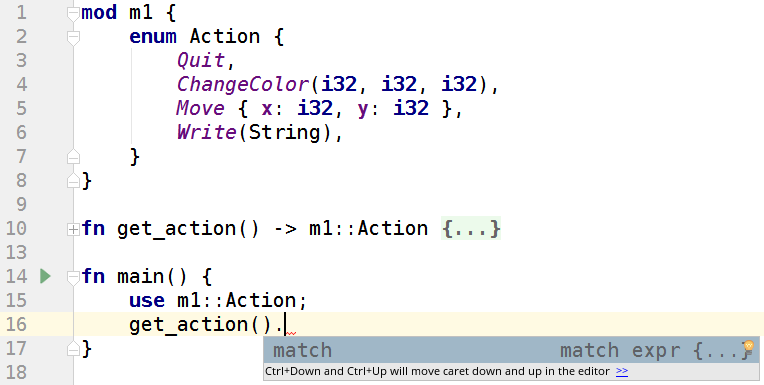
\includegraphics[scale = 0.6]{match_before.png}
\end{frame}

\begin{frame}
	\frametitle{Postfix tempaltes. Пример} 
	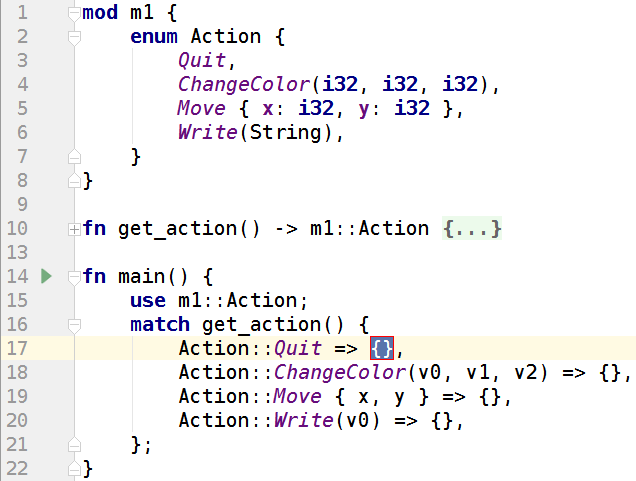
\includegraphics[scale = 0.6]{match_after.png}
\end{frame}


\begin{frame}
\frametitle{Упрощённое Psi-дерево} 
\centering
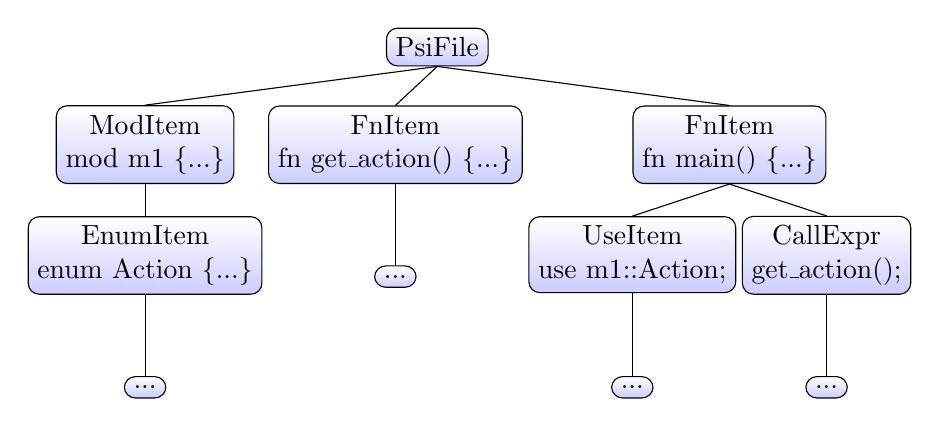
\begin{tikzpicture}[
	level distance = 4em,
	every node/.style = {
		shape=rectangle, rounded corners,
		draw, align=center,
		top color=white, bottom color=blue!20}]

	\Tree 
	[.PsiFile 
		[.{ModItem\\mod m1 \{...\}} [.{EnumItem\\enum Action \{...\}} ... ]]
		[.{FnItem\\fn get\_action() \{...\}} ... ]
		[.{FnItem\\fn main() \{...\}} 
			[.{UseItem\\use m1::Action;} ... ]
			[.{CallExpr\\get\_action();} ... ]
		]
	]
\end{tikzpicture}
	
\end{frame}

\begin{frame}
	\frametitle{Упрощённое поддерево ModItemElement} 
	{	
	\centering
		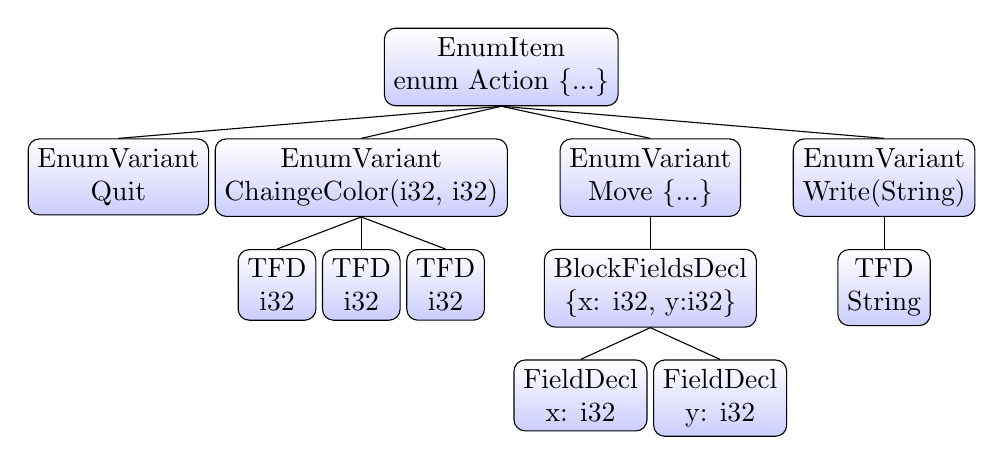
\begin{tikzpicture}[
		level distance = 4em,
		every node/.style = {
			shape=rectangle, rounded corners,
			draw, align=center,
			top color=white, bottom color=blue!20}]
		
		\Tree 
		[.{EnumItem\\enum Action \{...\}} 
			[.{EnumVariant\\Quit} ]
			[.{EnumVariant\\ChaingeColor(i32, i32)} 
				{TFD\\i32} {TFD\\i32} {TFD\\i32}
			]
			[.{EnumVariant\\Move \{...\}} 
				[.{BlockFieldsDecl\\\{x: i32, y:i32\}} 
					{FieldDecl\\x: i32}
					{FieldDecl\\y: i32}
				]
			]
			[.{EnumVariant\\Write(String)}
			{TFD\\String} 
			]
		]
		\end{tikzpicture}
	}
	\vfill
	TFD - TupleFieldDeclararion
	
\end{frame}

\begin{frame}
	\frametitle{Список Postfix templates} 
	\begin{itemize}
		\item if / else
		\item while / while not
		\item match
		\item paren 
		\item lambda
		\item assert, assert\_eq
		\item val ?
		\item for !!!!!!!!!!!!!!!
	\end{itemize}
\end{frame}

\begin{frame}
	\frametitle{Intentions} 
	\begin{itemize}
		\item Добавление ветви else к if
		\item Добавление/удаление {} вокруг single-expression
		\item Match to let if
	\end{itemize}
	\vfill
	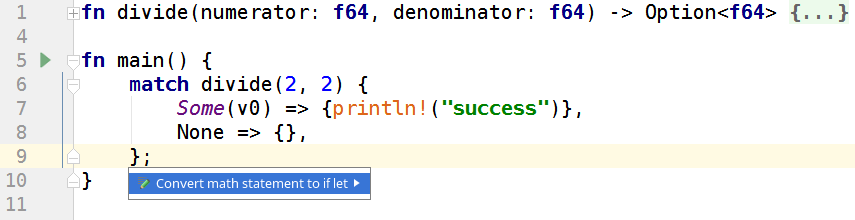
\includegraphics[scale = 0.4]{match2let_if_before.png}\\
	{
	\centering
	$\Downarrow$ \\
	}
	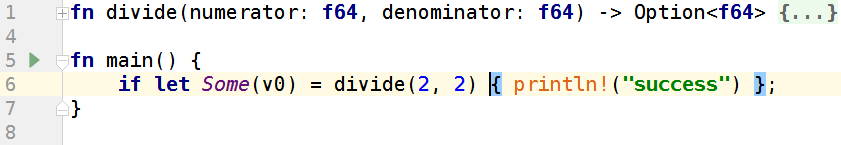
\includegraphics[scale = 0.4]{match2let_if_after.png}
\end{frame}

\begin{frame}
	\frametitle{Surround with...} 
	\begin{block}{Expression surround with}
		\begin{itemize}
			\item if
			\item while
			\item скобки ()
			\item отрицание !
		\end{itemize}
	\end{block}
	
	\begin{block}{Statements surround with}
		\begin{itemize}
			\item if
			\item while
			\item loop
			\item for
			\item скобки {}
		\end{itemize}
	\end{block}
\end{frame}

\begin{frame}
	\frametitle{Surround with...} 
	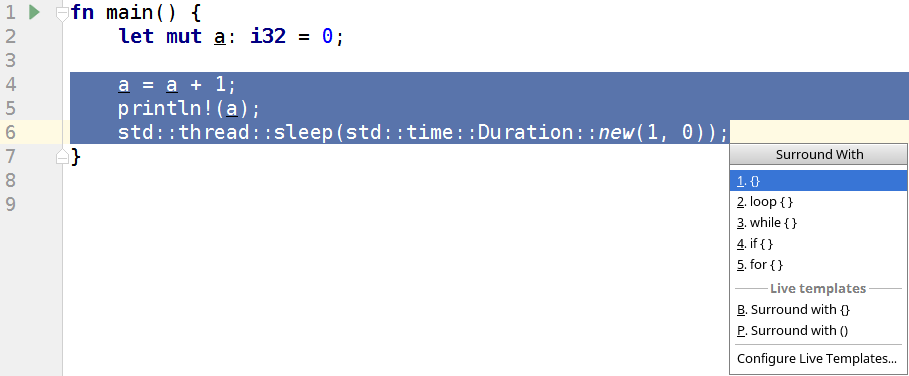
\includegraphics[scale = 0.4]{loop_before.png}\\
	{
		\centering $\Downarrow$ \\
	}
	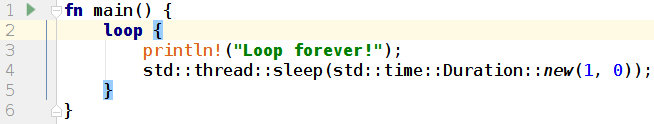
\includegraphics[scale = 0.4]{loop_after.png}
\end{frame}

\begin{frame}
	\frametitle{Технологии} 
	\begin{itemize}
		\item Rust
		\item Idea plugin API
		\item Kotlin
		\item GitHub
	\end{itemize}
\end{frame}

\end{document}
